% answers.tex —— 1993 年·新科目组·理科 · 参考答案与详细解析片段
% 由 tools/generate_projects.py 依来源总账自 1993/1993_数学真题_新科目组理_试题.md + 1993/1993_数学真题_新科目组理_解析正文.md + 1993/1993_数学真题_新科目组理_答案要点.md 生成，勿手改（改源 MD 后重跑）


\begin{gknotice}
\textbf{解析归属}：固定源 PDF 只有题面，没有答案页。以下推导依据固定题面形成，\textbf{非官方解析}；已由独立解题者在只读题面的条件下逐题盲核（题面 28 题无转录差异）。第 21 题的 \(f^{-1}(0)\) 记号按原像/零点集理解、第 28 题保留 \(\arg\) 约定分支，均在题面与答案要点中标注。原页疑点保留在题面中，不以推导结果反改原题。
\end{gknotice}

\begin{answer}
\gksolhead{1}{}

\textbf{题目}：

函数 $f(x)=\sin x+\cos x$ 的最小正周期是\mbox{（　　）}。

（A）$2\pi$　　（B）$2\sqrt2\pi$　　（C）$\pi$　　（D）$\dfrac\pi4$

\Needspace{4\baselineskip}
\textbf{解析}

$f(x)=\sqrt2\sin(x+\pi/4)$，非零正弦函数的最小正周期为 $2\pi$。

\gkanswer{答案：A}

\end{answer}
\begin{answer}
\gksolhead{2}{}

\textbf{题目}：

如果双曲线的焦距为 $6$，两条准线间的距离为 $4$，那么该双曲线的离心率为\mbox{（　　）}。

（A）$\dfrac32$　　（B）$\dfrac{\sqrt3}{2}$　　（C）$\dfrac{\sqrt6}{2}$　　（D）$2$

\Needspace{4\baselineskip}
\textbf{解析}

双曲线焦距 $2c=6$，故 $c=3$。两准线间距为 $2a/e=2a^2/c=4$，得 $a^2=6$，于是 $e=c/a=\sqrt6/2$。

\gkanswer{答案：C}

\end{answer}
\begin{answer}
\gksolhead{3}{}

\textbf{题目}：

和直线 $3x-4y+5=0$ 关于 $x$ 轴对称的直线的方程为\mbox{（　　）}。

（A）$3x+4y-5=0$　　（B）$3x+4y+5=0$

（C）$-3x+4y-5=0$　　（D）$-3x+4y+5=0$

\Needspace{4\baselineskip}
\textbf{解析}

关于 $x$ 轴对称时将原式中的 $y$ 换成 $-y$，得 $3x+4y+5=0$。

\gkanswer{答案：B}

\end{answer}
\begin{answer}
\gksolhead{4}{}

\textbf{题目}：

极坐标方程 $\rho=\dfrac4{3-5\cos\theta}$ 所表示的曲线是\mbox{（　　）}。

（A）焦点到准线距离为 $\dfrac45$ 的椭圆

（B）焦点到准线距离为 $\dfrac45$ 的双曲线右支

（C）焦点到准线距离为 $\dfrac43$ 的椭圆

（D）焦点到准线距离为 $\dfrac43$ 的双曲线右支

\Needspace{4\baselineskip}
\textbf{解析}

与焦点为极点的圆锥曲线标准式
$\rho=\dfrac{ed}{1-e\cos\theta}$ 对照，得 $e=5/3$、$ed=4/3$，故焦点到准线距离 $d=4/5$；因 $e>1$ 为双曲线，且选取右支。

\gkanswer{答案：B}

\end{answer}
\begin{answer}
\gksolhead{5}{}

\textbf{题目}：

$y=x^{3/5}$ 在 $[-1,1]$ 上是\mbox{（　　）}。

（A）增函数且是奇函数　　（B）增函数且是偶函数

（C）减函数且是奇函数　　（D）减函数且是偶函数

\Needspace{4\baselineskip}
\textbf{解析}

对实数按奇次根解释，$x^{3/5}=(\sqrt[5]x)^3$ 在实数上严格递增，且是奇函数。

\gkanswer{答案：A}

\end{answer}
\begin{answer}
\gksolhead{6}{}

\textbf{题目}：

$\displaystyle\lim_{n\to\infty}\dfrac{5n^2-1}{2n^2-n+5}$ 的值为\mbox{（　　）}。

（A）$-\dfrac15$　　（B）$-\dfrac52$　　（C）$\dfrac15$　　（D）$\dfrac52$

\Needspace{4\baselineskip}
\textbf{解析}

分子、分母同除以 $n^2$，极限为 $5/2$。

\gkanswer{答案：D}

\end{answer}
\begin{answer}
\gksolhead{7}{}

\textbf{题目}：

集合
$M=\left\{x\mid x=\dfrac{k\pi}{2}+\dfrac\pi4,\ k\in\mathbb Z\right\}$，
$N=\left\{x\mid x=\dfrac{k\pi}{4}+\dfrac\pi2,\ k\in\mathbb Z\right\}$，
则\mbox{（　　）}。

（A）$M=N$　　（B）$M\supseteq N$　　（C）$M\subseteq N$　　（D）$M\cap N=\varnothing$

\Needspace{4\baselineskip}
\textbf{解析}

$M$ 为所有奇数倍 $\pi/4$，$N$ 为所有整数倍 $\pi/4$，所以 $M\subseteq N$。

\gkanswer{答案：C}

\end{answer}
\begin{answer}
\gksolhead{8}{}

\textbf{题目}：

$\sin20^\circ\cos70^\circ+\sin10^\circ\sin50^\circ$ 的值是\mbox{（　　）}。

（A）$\dfrac14$　　（B）$\dfrac{\sqrt3}{2}$　　（C）$\dfrac12$　　（D）$\dfrac{\sqrt3}{4}$

\Needspace{4\baselineskip}
\textbf{解析}

\Needspace{5\baselineskip}
$\cos70^\circ=\sin20^\circ$，且
\nopagebreak[4]
\[
\sin10^\circ\sin50^\circ=\frac{\cos40^\circ-\cos60^\circ}{2}.
\]
与 $\sin^220^\circ=(1-\cos40^\circ)/2$ 相加得 $1/4$。

\gkanswer{答案：A}

\end{answer}
\begin{answer}
\gksolhead{9}{}

\textbf{题目}：

\Needspace{5\baselineskip}
参数方程
\nopagebreak[4]
\[
\begin{cases}
x=\cos\dfrac\theta2+\sin\dfrac\theta2,\\
y=\dfrac12(1+\sin\theta),
\end{cases}\quad(0<\theta<2\pi)
\]
表示\mbox{（　　）}。

（A）双曲线的一支，这支过点 $\left(1,\dfrac12\right)$

（B）抛物线的一部分，这部分过点 $\left(1,\dfrac12\right)$

（C）双曲线的一支，这支过点 $\left(-1,\dfrac12\right)$

（D）抛物线的一部分，这部分过点 $\left(-1,\dfrac12\right)$

\Needspace{4\baselineskip}
\textbf{解析}

\Needspace{5\baselineskip}
由参数式
\nopagebreak[4]
\[
x^2=(\cos\tfrac\theta2+\sin\tfrac\theta2)^2=1+\sin\theta=2y,
\]
轨迹在抛物线 $x^2=2y$ 上。$\theta=\pi$ 时取得 $(1,1/2)$，符合选项 B；端点 $\theta=2\pi$ 不在参数范围内，故不经过 $(-1,1/2)$。

\gkanswer{答案：B}

\end{answer}
\begin{answer}
\gksolhead{10}{}

\textbf{题目}：

若 $a\text{、}b$ 是任意实数，且 $a>b$，则\mbox{（　　）}。

（A）$a^2>b^2$　　（B）$\dfrac ba<1$

（C）$\lg(a-b)>0$　　（D）$\left(\dfrac12\right)^a<\left(\dfrac12\right)^b$

\Needspace{4\baselineskip}
\textbf{解析}

函数 $(1/2)^x$ 严格递减，故 $a>b$ 蕴含 $(1/2)^a<(1/2)^b$。

\gkanswer{答案：D}

\end{answer}
\begin{answer}
\gksolhead{11}{}

\textbf{题目}：

一动圆与两圆 $x^2+y^2=1$ 和 $x^2+y^2-8x+12=0$ 都外切，则动圆圆心轨迹为\mbox{（　　）}。

（A）圆　　（B）椭圆　　（C）双曲线的一支　　（D）抛物线

\Needspace{4\baselineskip}
\textbf{解析}

两定圆圆心分别为 $(0,0)$、$(4,0)$，半径分别为 $1$、$2$。若动圆半径为 $r>0$，圆心到两定圆圆心的距离分别为 $r+1$ 与 $r+2$，两距离之差恒为 $1$，小于两焦点间距 $4$，故轨迹为双曲线的一支。

\gkanswer{答案：C}

\end{answer}
\begin{answer}
\gksolhead{12}{}

\textbf{题目}：

圆柱轴截面的周长 $l$ 为定值，那么圆柱体积的最大值是\mbox{（　　）}。

（A）$\left(\dfrac l6\right)^3\pi$　　（B）$\dfrac19\left(\dfrac l2\right)^3\pi$

（C）$\left(\dfrac l4\right)^3\pi$　　（D）$2\left(\dfrac l4\right)^3\pi$

\Needspace{4\baselineskip}
\textbf{解析}

\Needspace{5\baselineskip}
设圆柱底半径为 $r$、高为 $h$，轴截面周长给出 $2h+4r=l$。体积
\nopagebreak[4]
\[
V=\pi r^2h=\pi r^2\left(\frac l2-2r\right)
\]
在 $r=l/6$ 时取最大值，此时 $h=l/6$，$V_{\max}=\pi(l/6)^3$。

\gkanswer{答案：A}

\end{answer}
\begin{answer}
\gksolhead{13}{}

\textbf{题目}：

$(\sqrt{x}+1)^4(x-1)^5$ 展开式中 $x^4$ 的系数为\mbox{（　　）}。

（A）$-40$　　（B）$10$　　（C）$40$　　（D）$45$

\Needspace{4\baselineskip}
\textbf{解析}

\Needspace{5\baselineskip}
\looseness=-1 令 $(\sqrt{x}+1)^4=\sum_{k=0}^4\binom4k x^{k/2}$。与 $(x-1)^5$ 相乘后，$x^4$ 项只可能来自 $k=0,2,4$，系数为
\nopagebreak[4]
\[
-\binom54+6\binom53-\binom52=-5+60-10=45.
\]

\gkanswer{答案：D}

\end{answer}
\begin{answer}
\gksolhead{14}{}

\textbf{题目}：

直角梯形的一个内角为 $45^\circ$，下底长为上底长的 $\dfrac32$，这个梯形绕下底所在的直线旋转一周所成的旋转体的全面积为 $(5+\sqrt2)\pi$，则旋转体的体积为\mbox{（　　）}。

（A）$2\pi$　　（B）$\dfrac{4+\sqrt2}{3}\pi$

（C）$\dfrac{5+\sqrt2}{3}\pi$　　（D）$\dfrac73\pi$

\Needspace{4\baselineskip}
\textbf{解析}

\Needspace{5\baselineskip}
设梯形高为 $h$、上底为 $u$、下底为 $b$。$b=3u/2$ 且斜边与底边夹角为 $45^\circ$，故 $b-u=h$，从而 $u=2h$、$b=3h$。旋转后为半径 $h$、长 $2h$ 的圆柱加高 $h$、底半径 $h$ 的圆锥；全面积为
\nopagebreak[4]
\[
\pi h^2+2\pi h(2h)+\pi h(\sqrt2h)=(5+\sqrt2)\pi h^2.
\]
由题设得 $h=1$，体积为 $2\pi+\pi/3=7\pi/3$。

\gkanswer{答案：D}

\end{answer}
\begin{answer}
\gksolhead{15}{}

\textbf{题目}：

已知 $a_1,a_2,\ldots,a_8$ 为各项都大于零的等比数列，公比 $q\ne1$，则\mbox{（　　）}。

（A）$a_1+a_8>a_4+a_5$

（B）$a_1+a_8<a_4+a_5$

（C）$a_1+a_8=a_4+a_5$

（D）$a_1+a_8$ 和 $a_4+a_5$ 的大小关系不能由已知条件确定

\Needspace{4\baselineskip}
\textbf{解析}

\Needspace{5\baselineskip}
令公比为 $q>0$，则
\nopagebreak[4]
\[
(a_1+a_8)-(a_4+a_5)=a_1(1-q^3)(1-q^4)>0
\]
对 $q>0,\ q\ne1$ 成立，所以 $a_1+a_8>a_4+a_5$。

\gkanswer{答案：A}

\end{answer}
\begin{answer}
\gksolhead{16}{}

\textbf{题目}：

设有如下三个命题：

甲：相交两直线 $l,m$ 都在平面 $\alpha$ 内，并且都不在平面 $\beta$ 内。

乙：$l,m$ 之中至少有一条与 $\beta$ 相交。

丙：$\alpha$ 与 $\beta$ 相交。

当甲成立时\mbox{（　　）}。

（A）乙是丙的充分而不必要的条件

（B）乙是丙的必要而不充分的条件

（C）乙是丙的充分且必要的条件

（D）乙既不是丙的充分条件又不是丙的必要条件

\Needspace{4\baselineskip}
\textbf{解析}

若 $\alpha,\beta$ 相交，记交线为 $g$。甲说明 $l,m$ 都在 $\alpha$ 内但都不与 $g$ 重合；二者不可能同时平行于 $g$，否则彼此平行而不能相交。因此至少一条与 $g$ 相交，也就与 $\beta$ 相交。反之若 $\alpha,\beta$ 不相交，则两平面平行，位于 $\alpha$ 的直线不与 $\beta$ 相交，乙不成立。因此乙与丙等价。

\gkanswer{答案：C}

\end{answer}
\begin{answer}
\gksolhead{17}{}

\textbf{题目}：

将数字 $1,2,3,4$ 填入标号为 $1,2,3,4$ 的四个方格里，每格填一个数字，则每个方格的标号与所填的数字均不相同的填法有\mbox{（　　）}。

（A）$6$ 种　　（B）$9$ 种　　（C）$11$ 种　　（D）$23$ 种

\Needspace{4\baselineskip}
\textbf{解析}

这是四元错排数，
$!4=4!(1-1+1/2!-1/3!+1/4!)=9$。

\gkanswer{答案：B}

\end{answer}
\begin{answer}
\gksolhead{18}{}

\textbf{题目}：

$\displaystyle\sin\left(\arccos\dfrac12+\arccos\dfrac13\right)=$\underline{\qquad\qquad}。

\Needspace{4\baselineskip}
\textbf{解析}

\Needspace{5\baselineskip}
\looseness=-1 设 $A=\arccos(1/2)$、$B=\arccos(1/3)$，则 $\sin A=\sqrt3/2$、$\sin B=2\sqrt2/3$，由和角公式得
\nopagebreak[4]
\[
\sin(A+B)=\frac{\sqrt3}{6}+\frac{2\sqrt2}{6}.
\]

\gkanswer{答案：\(\dfrac{\sqrt3+2\sqrt2}{6}\)}

\end{answer}
\begin{answer}
\gksolhead{19}{}

\textbf{题目}：

若双曲线 $\dfrac{x^2}{9k^2}-\dfrac{y^2}{4k^2}=1$ 与圆 $x^2+y^2=1$ 没有公共点，则实数 $k$ 的取值范围为\underline{\qquad\qquad}。

\Needspace{4\baselineskip}
\textbf{解析}

\Needspace{5\baselineskip}
令 $X=x^2$、$Y=y^2$，圆上有 $X+Y=1$、$0\le X\le1$。若两曲线相交，则
\nopagebreak[4]
\[
k^2=\frac X9-\frac Y4=\frac{13X-9}{36},
\]
其右端在 $[-1/4,1/9]$ 内。反之该表达式随 $X$ 连续取遍此区间，故有交点当且仅当 $0<k^2\le1/9$；$k=0$ 时原双曲线方程无定义。没有公共点等价于 $k^2>1/9$，即 $|k|>1/3$。

\gkanswer{答案：\(|k|>\dfrac13\)}

\end{answer}
\begin{answer}
\gksolhead{20}{}

\textbf{题目}：

从 $1,2,\ldots,10$ 这十个数中取出四个数，使它们的和为奇数，共有\underline{\qquad\qquad}种取法（用数字作答）。

\Needspace{4\baselineskip}
\textbf{解析}

和为奇数时，所取奇数个数为 $1$ 或 $3$。共有
$\binom51\binom53+\binom53\binom51=100$ 种。

\gkanswer{答案：\(100\)}

\end{answer}
\begin{answer}
\gksolhead{21}{}

\textbf{题目}：

设 $f(x)=4^x-2^{x+1}$，则 $f^{-1}(0)=$\underline{\qquad\qquad}。

\Needspace{4\baselineskip}
\textbf{解析}

$4^x-2^{x+1}=0$ 等价于 $2^{2x}=2^{x+1}$，故 $x=1$。

\gkanswer{答案：\(\{1\}\)（按 \(f^{-1}(0)\) 为原像/零点集理解）}

\end{answer}
\begin{answer}
\gksolhead{22}{}

\textbf{题目}：

建造一个容积为 $8\,\mathrm{m}^3$、深为 $2\,\mathrm m$ 的长方体无盖水池。如果池底和池壁的造价每平方米分别为 $120$ 元和 $80$ 元，那么水池的最低总造价为\underline{\qquad\qquad}元。

\Needspace{4\baselineskip}
\textbf{解析}

设池底边长为 $x,y$，则 $xy=8/2=4$。底面造价为 $480$ 元，四壁面积为 $4(x+y)$，壁面造价为 $320(x+y)$。由 $x+y\ge2\sqrt{xy}=4$，总造价至少 $480+1280=1760$ 元，正方形池底取等号。

\gkanswer{答案：\(1760\) 元}

\end{answer}
\begin{answer}
\gksolhead{23}{}

\textbf{题目}：

如图，$ABCD$ 是正方形，$E$ 是 $AB$ 的中点。如将 $\triangle DAE$ 和 $\triangle CBE$ 分别沿虚线 $DE$ 和 $CE$ 折起，使 $AE$ 与 $BE$ 重合，记 $A$ 与 $B$ 重合的点为 $P$，则面 $PCD$ 与面 $ECD$ 所成的二面角为\underline{\qquad\qquad}度。
\nopagebreak[4]
\begin{center}% 1993_新科目组_理科/figures/f1993_new_science_q23_fold.tex — 1993 年·新科目组·理科 第 23 题（折叠正方形示意）
%
% 【来源】`.work/phase4-b17/source/1993新科目组理.pdf`（SHA-256 14297950237f422e346d8c8a60ba0a9bb18d2ac4bcb69de4dabcb0ae2e83bd2d），第 1 页；
%   内容流 `q 1 0 0 1 901.783 516.913 cm` 段逐路径照录，
%   解析脚本 `.work/phase4-b17/probe/pdfparse_full.py`。
%
% 【坐标口径】源 PDF 用户空间（原点左下、y 向上）。本图本地坐标
%   (x,y) = (x_page − 901.783, y_page − 516.913)，1 单位 = 1 TeX pt。
%   线宽 0.398pt；虚线 [2.989 2.989] 0 d。
%
% 元素计数：实线 10 段（正方体四边、折叠后 D′C′/D′E′/C′E′/PE/PD′/PC′）+ 虚线 2 段（DE、CE）+ 9 个标签。
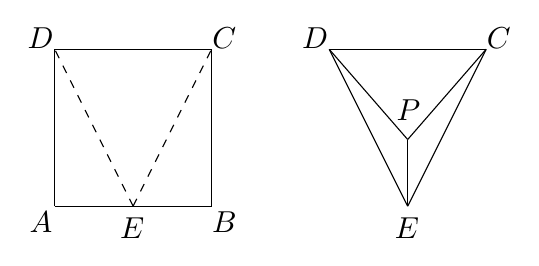
\begin{tikzpicture}[x=1pt, y=1pt,
    every node/.style={inner sep=0pt, font=\fontsize{10.5pt}{12.6pt}\selectfont}]
  \draw[line width=0.398pt] (0.000,0.000) -- (56.694,0.000);
  \draw[line width=0.398pt] (56.694,56.694) -- (56.694,0.000);
  \draw[line width=0.398pt] (56.694,56.694) -- (0.000,56.694);
  \draw[line width=0.398pt] (0.000,0.000) -- (0.000,56.694);
  \draw[line width=0.398pt] (99.214,56.694) -- (127.561,0.000);
  \draw[line width=0.398pt] (155.907,56.694) -- (127.561,0.000);
  \draw[line width=0.398pt] (155.907,56.694) -- (99.214,56.694);
  \draw[line width=0.398pt] (127.561,24.095) -- (127.561,0.000);
  \draw[line width=0.398pt] (127.561,24.095) -- (99.214,56.694);
  \draw[line width=0.398pt] (127.561,24.095) -- (155.907,56.694);
  % 虚线：正方形内 DE、CE（折痕）
  \draw[line width=0.398pt, dash pattern=on 2.989pt off 2.989pt] (28.347,0.000) -- (0.000,56.694);
  \draw[line width=0.398pt, dash pattern=on 2.989pt off 2.989pt] (28.347,0.000) -- (56.694,56.694);
  \node[anchor=center] at (-5.070,60.770) {$D$};
  \node[anchor=center] at (61.250,60.770) {$C$};
  \node[anchor=center] at (-4.930,-5.780) {$A$};
  \node[anchor=center] at (28.050,-7.820) {$E$};
  \node[anchor=center] at (61.360,-5.780) {$B$};
  \node[anchor=center] at (94.140,60.770) {$D$};
  \node[anchor=center] at (160.470,60.770) {$C$};
  \node[anchor=center] at (127.830,34.700) {$P$};  % 相对源中心上移 2.49pt、右移 1.0pt，避开 D–P 边
  \node[anchor=center] at (127.260,-7.820) {$E$};
\end{tikzpicture}
%
% 【自验结果】探针：坐标逐点照录内容流；与 400 dpi 渲染并排比对（标签位置取 pdftotext -bbox 中心）。
\end{center}
\nopagebreak[4]
\Needspace{4\baselineskip}
\textbf{解析}

角度不受缩放影响，取正方形边长为 $2$，令
$E=(0,0,0)$、$A=(-1,0,0)$、$B=(1,0,0)$、$D=(-1,2,0)$、$C=(1,2,0)$。
\Needspace{5\baselineskip}
折叠后 $PE=1$ 且 $PD=PC=2$。由对称性令 $P=(0,y,z)$，则
\nopagebreak[4]
\[
y^2+z^2=1,\qquad 1+(y-2)^2+z^2=4,
\]
解得 $y=1/2,\ z^2=3/4$。在垂直于 $CD$ 的截面中，取 $O$ 为 $CD$ 中点，则
$\overrightarrow{OE}=(0,-2,0)$、$\overrightarrow{OP}=(0,-3/2,\sqrt3/2)$，
故二面角的较小角满足 $\cos\theta=\sqrt3/2$，所以 $\theta=30^\circ$。坐标只为验证折叠长度关系，不把原图示意比例当作题设数据。

\gkanswer{答案：\(30^\circ\)}

\end{answer}
\begin{answer}
\gksolhead{24}{}

\textbf{题目}：

已知 $f(x)=\log_a\dfrac{1+x}{1-x}\ (a>0,\ a\ne1)$。

(1) 求 $f(x)$ 的定义域；

(2) 判断 $f(x)$ 的奇偶性并予以证明；

(3) 求使 $f(x)>0$ 的 $x$ 取值范围。

\Needspace{4\baselineskip}
\textbf{解析}

\gksubpart{(1)}

需有 \(\dfrac{1+x}{1-x}>0\)，解得 \(-1<x<1\)，故定义域为 \((-1,1)\)。

\gksubpart{(2)}

\Needspace{5\baselineskip}
对定义域内任意 \(x\)，
\nopagebreak[4]
\[
f(-x)=\log_a\frac{1-x}{1+x}=-\log_a\frac{1+x}{1-x}=-f(x),
\]
故 \(f(x)\) 为奇函数。

\gksubpart{(3)}

当 \(a>1\) 时，\(f(x)>0\) 当且仅当 \(\dfrac{1+x}{1-x}>1\)，结合定义域得 \(0<x<1\)；当 \(0<a<1\) 时，\(f(x)>0\) 当且仅当 \(0<\dfrac{1+x}{1-x}<1\)，结合定义域得 \(-1<x<0\)。

\gkanswer{答案（1）：定义域 \((-1,1)\)}

\gkanswer{答案（2）：奇函数（证明见解析）}

\gkanswer{答案（3）：\(a>1\) 时 \(x\in(0,1)\)；\(0<a<1\) 时 \(x\in(-1,0)\)}

\end{answer}
\begin{answer}
\gksolhead{25}{}

\textbf{题目}：

已知数列
$\dfrac{8\cdot1}{1^2\cdot3^2},\ \dfrac{8\cdot2}{3^2\cdot5^2},\ \ldots,\ \dfrac{8n}{(2n-1)^2(2n+1)^2},\ \ldots$，$S_n$ 为其前 $n$ 项和。
计算得 $S_1=\dfrac89,\ S_2=\dfrac{24}{25},\ S_3=\dfrac{48}{49},\ S_4=\dfrac{80}{81}$。观察上述结果，推测出计算 $S_n$ 的公式，并用数学归纳法加以证明。

\Needspace{4\baselineskip}
\textbf{解析}

\textbf{猜想：$S_n=1-\dfrac1{(2n+1)^2}$。}

\Needspace{5\baselineskip}
通项可裂项为
\nopagebreak[4]
\[
\frac{8n}{(2n-1)^2(2n+1)^2}
=\frac1{(2n-1)^2}-\frac1{(2n+1)^2}.
\]
\Needspace{5\baselineskip}
因此前 $n$ 项相加望远镜消去，得 $S_n=1-1/(2n+1)^2$。也可用归纳法：$n=1$ 时成立；若 $S_n=1-1/(2n+1)^2$，则利用上面的裂项式可得
\nopagebreak[4]
\[
S_{n+1}=S_n+\frac1{(2n+1)^2}-\frac1{(2n+3)^2}
=1-\frac1{(2n+3)^2},
\]
故对一切正整数 $n$ 成立。

\gkanswer{答案：\(S_n=1-\dfrac{1}{(2n+1)^2}\)}

\end{answer}
\begin{answer}
\gksolhead{26}{}

\textbf{题目}：

已知：平面 $\alpha\cap$ 平面 $\beta=$ 直线 $a$。$\alpha,\beta$ 同垂直于平面 $\gamma$，又同平行于直线 $b$。求证：(1) $a\perp\gamma$；(2) $b\perp\gamma$。

\Needspace{4\baselineskip}
\textbf{解析}

\textbf{证明。}

两平面 $\alpha,\beta$ 都垂直于 $\gamma$，故其交线 $a$ 垂直于 $\gamma$，得 (1)。又 $b$ 同时平行于 $\alpha,\beta$，所以其方向平行于两平面的交线 $a$；由 $a\perp\gamma$ 得 $b\perp\gamma$，得 (2)。

\gkanswer{答案：两个结论均成立（两平面互相垂直、两直线互相垂直）}

\end{answer}
\begin{answer}
\gksolhead{27}{}

\textbf{题目}：

在面积为 $1$ 的 $\triangle PMN$ 中，$\tan\angle PMN=\dfrac12,\ \tan\angle MNP=-2$。建立适当的坐标系，求以 $M,N$ 为焦点且过点 $P$ 的椭圆方程。

\Needspace{4\baselineskip}
\textbf{解析}

令 $M=(-c,0)$、$N=(c,0)$，中点为原点，$MN$ 为 $x$ 轴。设 $\angle PMN=A$、$\angle MNP=B$。由正切及角的范围可得
$\sin A=1/\sqrt5,\ \cos A=2/\sqrt5,\ \sin B=2/\sqrt5,\ \cos B=-1/\sqrt5$，故
$\sin\angle MPN=\sin(A+B)=\sin A\cos B+\cos A\sin B=3/5$。
\Needspace{5\baselineskip}
设三角形外接圆直径为 $k$，正弦定理给出
\nopagebreak[4]
\[
PN=\frac{k}{\sqrt5},\quad PM=\frac{2k}{\sqrt5},\quad MN=\frac{3k}{5}.
\]
\Needspace{5\baselineskip}
面积条件
\nopagebreak[4]
\[
1=\frac12 PM\cdot PN\sin P=\frac{3k^2}{25}
\]
\Needspace{5\baselineskip}
给出 $k=5/\sqrt3$，所以 $MN=\sqrt3$、$c=\sqrt3/2$。过 $P$ 且以 $M,N$ 为焦点的椭圆满足 $2a=PM+PN=\sqrt{15}$，于是 $a^2=15/4$、$b^2=a^2-c^2=3$。所求方程为
\nopagebreak[4]
\[
\frac{x^2}{15/4}+\frac{y^2}{3}=1.
\]

\gkanswer{答案：\(\dfrac{x^2}{15/4}+\dfrac{y^2}{3}=1\)}

\end{answer}
\begin{answer}
\gksolhead{28}{}

\textbf{题目}：

\looseness=-1 设复数 $z=\cos\theta+i\sin\theta\ (0<\theta<\pi)$，
$\omega=\dfrac{1-(\overline z)^4}{1+z^4}$，并且 $|\omega|=\dfrac{\sqrt3}{3}$，$\arg\omega<\dfrac\pi2$，求 $\theta$。

\Needspace{4\baselineskip}
\textbf{解析}

\textbf{原题记号有待核。}

\Needspace{5\baselineskip}
令 $z=e^{i\theta}$，则
\nopagebreak[4]
\[
\omega=\frac{1-e^{-4i\theta}}{1+e^{4i\theta}}
=i e^{-4i\theta}\tan2\theta.
\]
模长条件给出 $|\tan2\theta|=1/\sqrt3$，在 $0<\theta<\pi$ 内候选为
$\theta=\pi/12,5\pi/12,7\pi/12,11\pi/12$。对应 $\omega$ 的辐角分别为 $\pi/6,-\pi/6,\pi/6,-\pi/6$（模 $2\pi$ 意义下）。若 $\arg$ 指值域 $[0,2\pi)$ 的辐角，则满足不等式的是 $\theta=\pi/12,7\pi/12$；若采用主辐角值域 $(-\pi,\pi]$，四个候选都满足。原卷未声明约定，故答案保持条件化，待独立核对原题惯例。

\gkanswer{答案：原题无唯一解集：主值 \((-\pi,\pi]\) 下四个候选均满足，\([0,2\pi)\) 下仅 \(\theta=\dfrac{\pi}{12},\dfrac{7\pi}{12}\)}

\end{answer}